\documentclass{llncs}
\usepackage{graphicx}
\usepackage{hyperref}
\usepackage{mathpartir}
\usepackage{subcaption}
\usepackage{textcomp}
\usepackage{wrapfig}

\newcommand{\lerna}{\textsc{Lerna}}
\newcommand{\z}[1]{\textsc{Z3}}
\newcommand{\mizarlarge}{\textit{M40k}}
\newcommand{\mizarsmall}{\textit{M2k}}
\begin{document}
\title{A Neural, Parallel Theorem Prover*}
\author{
	Michael Rawson*\orcidID{0000-0001-7834-1567} \and
	Giles Reger
}
\institute{
	University of Manchester, UK\\
	\email{michael@rawsons.uk}, \email{giles.reger@manchester.ac.uk}
}
\maketitle

\begin{abstract}
	We present a prototype of a neurally-guided automatic theorem prover for first-order logic with equality.
	The prototype uses a neural network trained on previous proof search attempts to evaluate subgoals based directly on their structure, and hence bias proof search toward success.
	An existing first-order theorem prover is employed to dispatch easy subgoals and prune branches which cannot be solved.
	Exploration of the search space is asynchronous with respect to both the evaluation network and the existing prover, allowing for efficient batched neural network execution and for natural parallelism within the prover.
	Evaluation on the MPTP dataset shows that the prover can improve with learning.
\keywords{ATP \and Graph Convolutional Network \and Tableaux \and MCTS}
\end{abstract}

%%%%%%%%%%%%%%%%%%%%%%%%%%%%%%%%%%%%%%%%%%%%%%%%%%%%%%%%%%%%%%
\section{Introduction}
Recent advances~ in neural network systems allow for processing graph-structured data in a neural context.
Graphs are a natural representation for logical formulae as found in automatic theorem provers (ATPs), suggesting a new breed of \emph{neural ATP} in which proof search is guided by a neural black-box acting as ``mathematician's intuition''.
However, in practice there are several implementation issues~\cite{lerna-discussion} which must be avoided in order for neural systems to integrate with efficient traditional ATPs:
\begin{enumerate}
	\item Proof state in such systems may be very large, such as in saturation-based provers, leading to training data which is impractical to learn from and slow to evaluate.
	\item Data structures employed may be very opaque or ``unnatural'', containing artifice designed for efficiency rather than natural comprehension by a neural network.
	\item Systems may be very sensitive to latency, which can result in the introduction of neural guidance systems crippling prover throughput and hence performance.
\end{enumerate}
%
Attempting to solve these issues with a novel prover architecture, and exploring several options to improve overall efficiency, the prototype system \lerna{}\footnote{\textbf{Le}arning to \textbf{R}eason with \textbf{N}eural \textbf{A}rchitectures. Lerna is also the lair of the mythical many-headed beast \textsc{Hydra}.} takes an alternative step toward useful neural automatic theorem provers.

%%%%%%%%%%%%%%%%%%%%%%%%%%%%%%%%%%%%%%%%%%%%%%%%%%%%%%%%%%%%%%
\section{Background}

We assume basic familiarity with first-order logic, theorem proving, and  neural networks~\cite{neural-survey}.

\subsection{Logic and Theorem Proving}

\paragraph{First-Order Logic}

\lerna{} works with formulas in standard first-order logic with equality. Terms $t$ and formulas $\phi$ are recursively defined as follows
\[
\begin{array}{ll}
t = & x \mid f\left(t_1, \ldots, t_n\right) \mid c \\
\phi  =  & \top \mid \bot \mid t_1 = t_2 \mid p\left(t_1, \ldots, t_n\right) \mid \phi_1 \Rightarrow \phi_2 \mid \phi_1 \equiv \phi_2\mid \neg \phi \mid \\ &   \phi_1 \wedge \ldots \wedge \phi_n \mid \phi_1  \vee \ldots \vee \phi_n \mid \forall x. \phi \mid \exists x. \phi
\end{array}
\]
where $x$ is a variable, $f$ is a $n$-ary function symbol, $c$ is a constant, and $p$ is a $n$-ary predicate symbol. Their meaning is defined as usual.

%A formula is either true \(\top\), false \(\bot\), an equality between terms \(t_1 = t_2\), a predicate applied to terms \(p\left(t_1, t_2, \ldots, t_n\right)\), where \(p\) is an \(n\)-ary predicate symbol, a negated formula \(\lnot \phi\), an impliciation \(\phi_1 \Rightarrow \phi_2\), or equivalences \(\phi \equiv \psi\).
%Conjunctions \(\phi_1 \wedge \phi_2 \wedge \ldots \wedge \phi_n\) or disjunctions \(\phi_1 \vee \phi_2 \vee \ldots \vee \phi_n\).
%Universal or existential quantifiers \(\forall x. \phi, \exists x. \phi\).


\paragraph{Modern Automatic Theorem Provers}
An automated theorem prover (ATP) is a system able to automatically establish whether a formula (in first-order logic) is \emph{satisfiable} or \emph{unsatisfiable}; although, given the undecidability of this problem, ATPs may also return \emph{unknown}. Both saturation-based provers (e.g. E~\cite{E}, iProver~\cite{iProver}, Vampire~\cite{Vampire}) and SMT solvers (e.g. CVC4~\cite{CVC4} and Z3~\cite{Z3}) utilise efficient proof calculi combined with highly-configurable search routines in order to explore a large search space efficiently.
%Generally, the search space in these systems slowly at first, then increases rapidly, leading to the maxim that a proof is typically found quickly or not at all.
%Portfolio modes~\cite{portfolio} are therefore employed in order to achieve good performance on a large set of practically-useful problems, such as those found in TPTP~\cite{TPTP}.

\subsection{Machine Learning and Theorem Proving}
Despite the efficiency of modern ATP systems, they can still spend time exploring areas that a human mathematician would discard, and tuning such systems is, in general, extremely difficult~\cite{portfolio}.
This has led to the application of machine-learning techniques, with the eventual aim of an ``intelligent'' theorem prover able to learn from past experience to develop an intuition, discard uninteresting search space, and tune performance in a more principled way.

Previous work has focussed on premise selection~\cite{DeepMath,MaSh,MaLARea,formula-graph}, static strategy selection~\cite{Bridge,MaLeS,E-MaLeS}, dynamic (run-time) strategy selection~\cite{dynamic-strategy-priority} and more recently, direct proof guidance~\cite{MaLeCoP,FEMaLeCoP,rlCoP,ENIGMA,DNGPS}.
Proof guidance typically involves a form of machine-learned \emph{heuristic} which biases proof search in some way, allowing the prover to avoid parts of the search space deemed uninteresting by the heuristic.

Much previous work on integrating machine-learned heuristics into automatic theorem provers has relied on hand-engineered features~\cite{MaLeCoP,FEMaLeCoP,rlCoP} or other embedding methods~\cite{ENIGMA}, which have the advantage of simplicity and relative efficiency, but do not encode all information available.
By contrast, a neural method which takes into account all information (as utilised in this work) should allow for greater precision in proof guidance systems.
Deep Network Guided Proof Search (DNGPS)~\cite{DNGPS} is an example of previous work in this area, which integrated a deep neural guidance system into the saturation-based prover E~\cite{E}.
DNGPS achieved successful results, but suffered from the latency introduced into the system by the neural heuristic: despite processing only a reduced amount of the available proof state, the reduction in throughput necessitated a two-phase approach in which the prover was neurally-guided in the first phase, before falling back to traditional proof search in the second.

\paragraph{rlCoP} The rlCoP system~\cite{rlCoP} is a connection-based reinforcement-learning prover which is not presently neurally-guided, but takes a similar approach to that taken in this paper and achieves impressive results.

\paragraph{Neural Networks for Formulae}
Neural networks are well-known tools for supervised learning~\cite{neural-survey}, and combined with trainable convolution/pooling operators are suitable for processing large-scale data such as images~\cite{cnn}.

Processing structured data such as logical formulae is a relatively new domain for neural networks.
Some work attempts to use unstructured representations of such formulae, such as text, or build entirely-new models for a specific logic~\cite{logical-entailment}, whereas others attempt to re-use neural techniques for generic structures such as trees~\cite{logical-tree}.
A promising direction in this area is recent research on neural methods working with graphs~\cite{graph-cnn,gcn,gcn-relational}, which have already been applied to premise selection~\cite{formula-graph}.
Graph neural networks tend to include network layers inspired by convolution operators in image-processing networks, combining information from neighbouring nodes (pixels).
For example, the Graph Convolutional Network~\cite{gcn} includes the following convolution layer, where \(H_i\) is the network output at layer \(i\), \(\bar{A}\) is the self-connected adjacency matrix, \(\bar{D}\) is the diagonal node degree matrix of \(\bar{A}\), \(W_i\) is a trainable weight matrix and \(\sigma\) is a non-linear activation function:
\[
	H_{i + 1} = \sigma\left(\bar{D}^{-\frac{1}{2}}\bar{A}\bar{D}^{-\frac{1}{2}}H_iW_i\right)
\]

\paragraph{The MPTP Problem Set}
For training and evaluation purposes a set of problems exported from the Mizar Mathematical Library~\cite{mizar} by the MPTP~\cite{MPTP} system are used.
Urban et al.~\cite{rlCoP} took a subset\footnote{\url{https://github.com/JUrban/deepmath/blob/master/M2k_list}} of the large \mizarlarge{} problem set (containing 32,524 problems) and called it \mizarsmall{} (containing 2004 problems).

%%%%%%%%%%%%%%%%%%%%%%%%%%%%%%%%%%%%%%%%%%%%%%%%%%%%%%%%%%%%%%
\section{Design}
\label{section:Design}
In order to achieve the goal of a neural theorem prover without the disadvantages associated with neural approaches, a new design of theorem prover is required.
Popular calculi used in existing ATPs tend to be unfriendly to neural guidance.
For such a system, we require the following from the calculus:
\begin{enumerate}
        \item \emph{Proof state must be small.} Attempting to evaluate large proof states structurally requires a lot of computation and resources. Saturation-based provers can have very large proof states, for example.
        \item \emph{Evaluation of states must be possible in parallel.} Machine-learning algorithms operate more efficiently in batches. Tree-based approaches (tableau \emph{etc.}) lend themselves to this, whereas saturation provers are inherently sequential.
        \item \emph{Subgoals must be independent and self-contained.} If the prover has a notion of (sub-)goals which must be dispatched (such as in tableau provers), these should be independent of the rest of the search space.%, without e.g. unifiers. 
        Otherwise, the learning system is trying to learn while blind to the context of the search.
	\item \emph{Subgoals must be intelligible.} Adding ``noise'' such as clausification obscures the original intuition behind a goal, at least for human observers. While this is not necessarily the case for machine-learning algorithms, it seems likely that removing structure and adding artefacts will reduce model performance.
\end{enumerate}
We therefore implement a refutation prover based on a first-order tableaux calculus without unification, on non-clausal formulae.
Each goal in this case is the set of formulae present on the tableau branch.
In this context, proof state is small (only the current branch), evaluation of states is possible in parallel, each branch is independent and contains all information required, and all available structure from the original problem is kept.

\subsection{Search}
In the calculus (see Section \ref{section:Calculus}) for this prover, there are two branching factors: each goal has a set of possible inferences, and each inference contains a set of possible sub-goals.
To prove a goal, at least one inference must be proved.
To prove an inference, all the inferences' sub-goals must be proved (e.g. shown to be unsatisfiable).
A simple optimisation is that sub-goals may be shared between inferences, so search becomes a directed acyclic graph, alternating between goals and inferences (illustrated in Fig.~\ref{fig:search}).

%\begin{figure}[t]
\begin{wrapfigure}[12]{r}{0.5\textwidth} 
\vspace{-26pt}
	\centering
	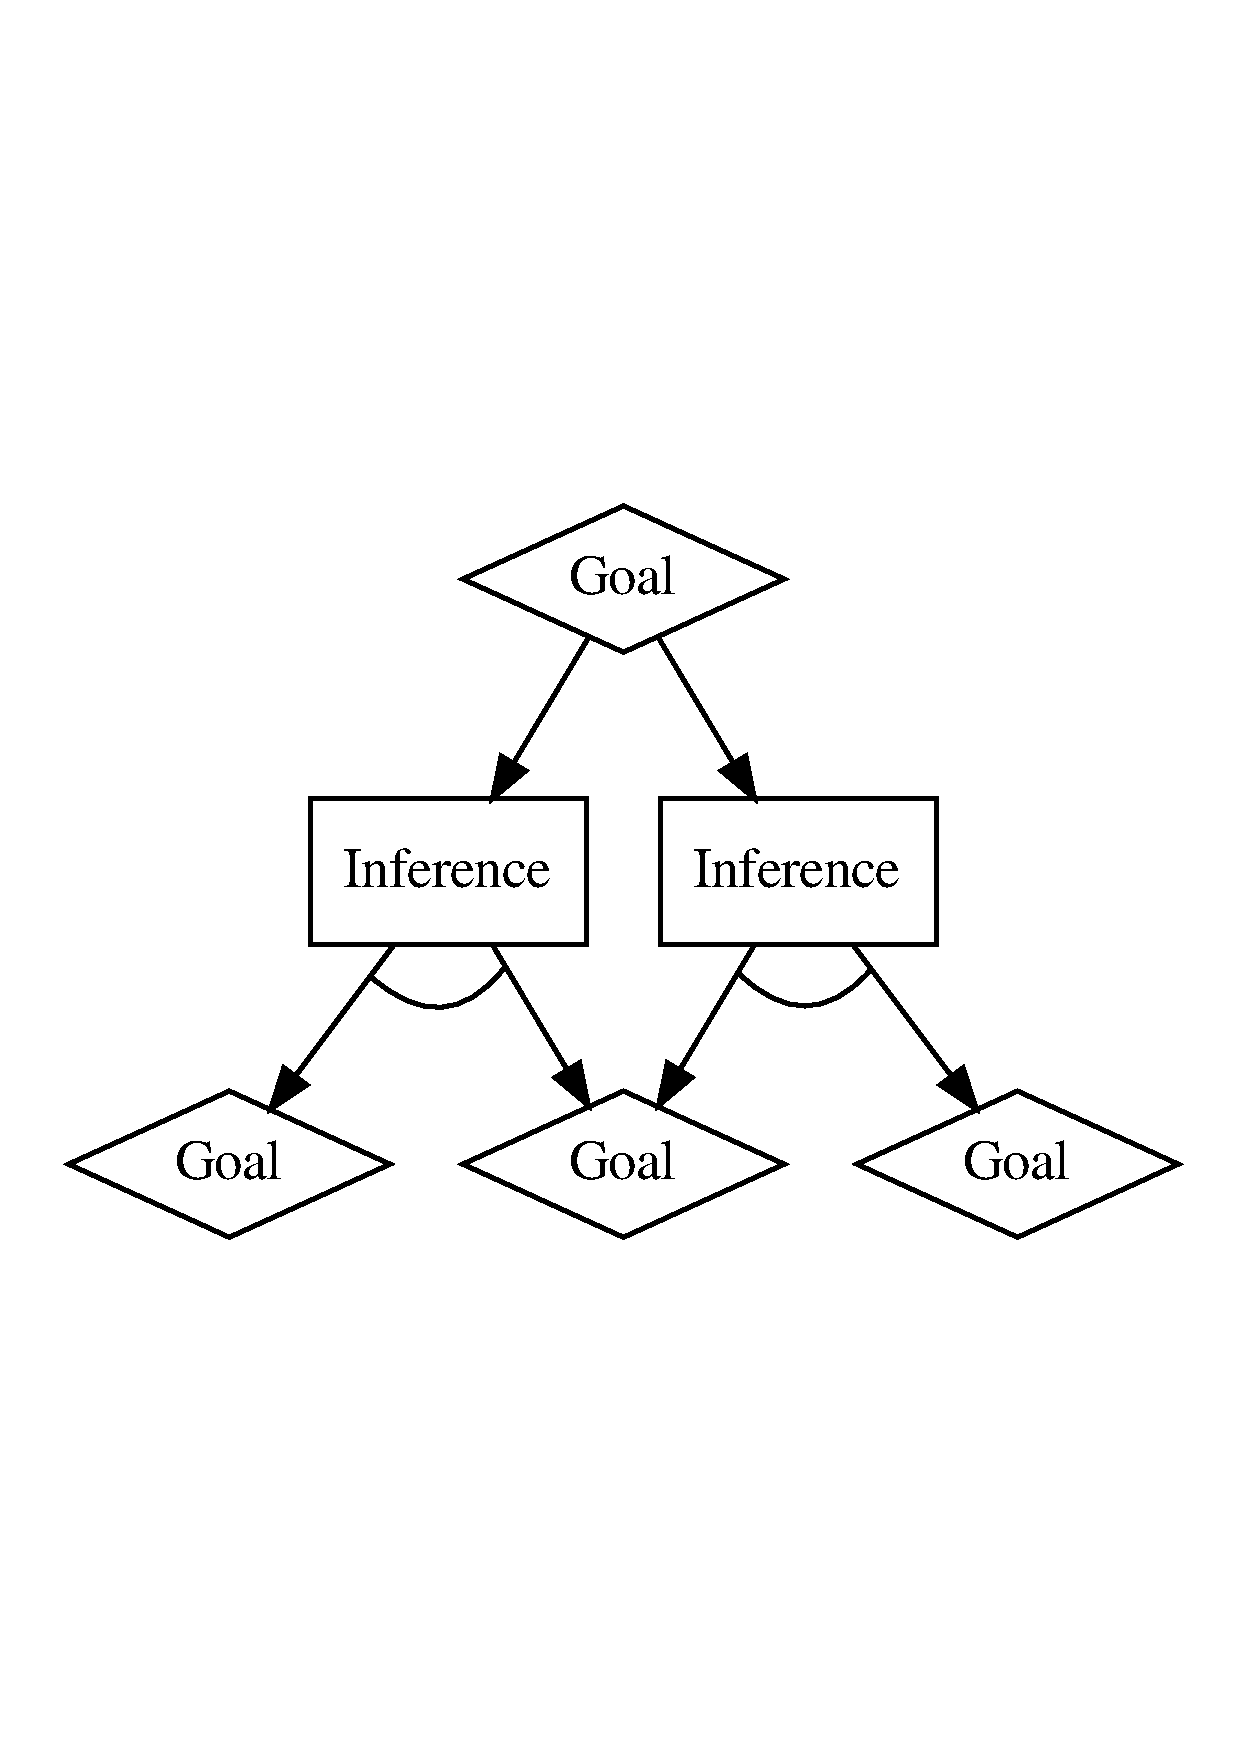
\includegraphics[width=0.9\linewidth]{search2.pdf}
	\caption{Search in the \lerna{} system, showing shared sub-goals.\label{fig:search}}
\end{wrapfigure}	
%\end{figure}

Now the search graph can be explored: in each step, a leaf (goal) node is selected for expansion, and all resulting inferences and sub-goals are added to the graph.
If a goal has no possible inferences, it is satisfiable and can be removed from the search space.
On the other hand, if a goal is trivial (i.e. contains a contradiction), it is unsatisfiable and can be marked as proven.
This idea is lifted to inferences: if an inference contains any satisfiable sub-goal, it too is satisfiable, whereas if an inference contains all unsatisfiable goals, it is unsatisfiable.
Proof search continues until the timeout is reached or the root goal is shown to be (un-)satisfiable.
In order to dispatch trivial sub-goals quickly, an existing fast \emph{oracle} ATP is used (see Section \ref{section:oracle}).
This may mark goals as (un-)satisfiable, at which point no further exploration is required.

Search is biased by heuristic evaluation.
The neural heuristic function (see Section \ref{section:heuristic}) evaluates each goal and assigns a score corresponding to whether the network believes that the goal is satisfiable or unsatisfiable.
In order to balance exploitation of promising directions and exploration of all parts of the search space, a principled UCT-based search algorithm is used, as in MonteCoP~\cite{MonteCoP}.
At each sub-goal $g$, the prover chooses the inference $i$ and subgoal $sg$ with the maximal expression
\[
{\sf max}_{i \in {\sf inferences}(g)}  	{\sf min}_{sg \in {\sf subgoals}(i)} \left ( {\sf score}(sg) + c~\sqrt{\frac{\ln {\sf visits}(g)}{{\sf visits}(sg)}} \right )  
\]
where ${\sf score}$ gives the heuristic score, ${\sf visits}$ gives the total number of visits to that node so far, and \(c\) is the exploration parameter (theoretically \(\sqrt{2}\)). This prioritises subgoals considered satisfiable by the heuristic as establishing satisfiability makes the subgoals redundancy, allowing them to be pruned.



\subsection{Architecture and Prototype Implementation}
The system aims to consume all available CPU and GPU resources as efficiently as possible.
To that end, proof search is asynchronous: the search algorithm generates new sub-goals, which are placed on two separate queues: one for the oracle ATP, another for heuristic evaluation.
Proof search then continues elsewhere, while the oracle ATP is called in parallel on each sub-goal (consuming all available CPU) while the heuristic consumes batches of subgoals, efficiently utilising the available computational resource.
As information flows backwards from these processes, the search process updates its information about a given sub-goal and propagates that information upwards to the sub-goal's parent inferences, to influence future proof search: see Fig. \ref{figure:architecture}.

\begin{figure}[t]
	\centering
	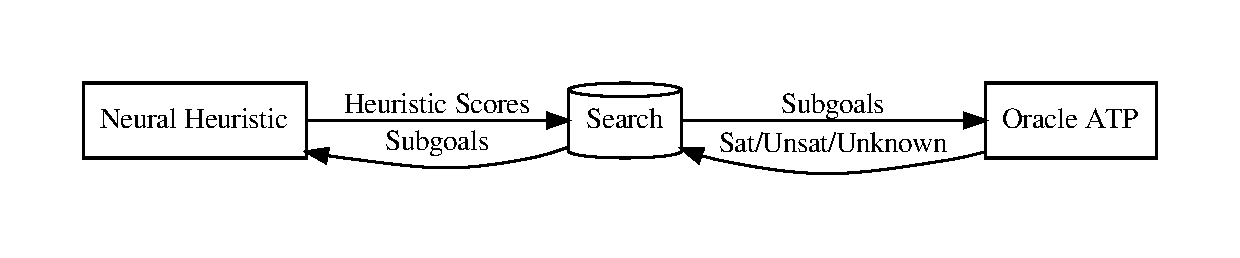
\includegraphics[width=0.8\linewidth]{architecture}
	\caption{Illustrating information-flow in the system.}
	\label{figure:architecture}
\end{figure}

%\subsection{}

The prototype implementation (minus the heuristic) %was built in the Rust programming language.% was chosen to implement the main prover , for its memory and thread-safety guarantees, as well as its support for managing memory allocation and algebraic datatypes.
%The implementation 
is currently just under 3,000 lines of Rust, not including \z3{}, the TPTP format parser or the implementation of perfect sharing.
Python 3 was used for the heuristic due to the large number of libraries available for neural network implementation in Python.
The heuristic is implemented as a server, communicating with the main prover via a TCP socket.
In principle this allows for the heuristic to be a shared resource with a centralised heuristic server, or a load-balanced cluster.

%%%%%%%%%%%%%%%%%%%%%%%%%%%%%%%%%%%%%%%%%%%%%%%%%%%%%%%%%%%%%%
\section{Calculus}
\label{section:Calculus}
The proof calculus used in the above architecture may be extremely general: in fact, any function from goals to a finite set of possible inferences (themselves finite sets of sub-goals) will suffice, as long as each goal remains independent of any other such that the heuristic function can process all available information.  If the inference system is complete, there are no additional constraints such as orderings or fairness to ensure the completeness of the prover, as the balanced search algorithm (see Section \ref{section:Design}) will ensure this.

\lerna{} presently implements a refutation tableaux calculus~\cite{handbook-of-automated-reasoning} without unification.
The calculus described is deliberately na\"ive in order to easily satisfy the design constraints given above, but may be replaced by a stronger calculus in the future. 
A na\"ive calculus is not necessarily a problem as the heuristic should select promising areas to explore and ignore uninteresting sub-goals.
However, a more efficient calculus would improve performance where the heuristic fails.

\paragraph{Refutation Tableaux}
In order to show a conjecture \(C\) from a set of axioms \(A_i\), it suffices to negate \(C\) and the show that the resulting conjunction \(A_1 \wedge A_2 \wedge \ldots \wedge \lnot C\) is unsatisfiable.
A set of inference rules of the form
\begin{mathpar}
	\inferrule{\Gamma_1 \\ \Gamma_2 \\ \ldots \\ \Gamma_n}{\Delta}
\end{mathpar}
where \(\Gamma_i, \Delta\) are sets of formulae and \(\lnot\left(\Gamma_1 \wedge \Gamma_2 \wedge \ldots \Gamma_n\right) \Rightarrow \lnot \Delta\) is an unconditional tautology, form a refutation calculus.
Proofs in this calculus can be expressed by closed trees of inference rules.

\begin{figure}[t]
	\centering
	\begin{mathpar}
		\inferrule[contradiction]{ }{\phi, \lnot \phi, \Gamma}\and
		\inferrule[equal]{t = s, \phi\left[t/s\right], \Gamma}{t = s, \phi, \Gamma}\and
		\inferrule[implies]{\lnot \phi, \psi, \Gamma}{\phi \Rightarrow \psi, \Gamma}\and
		\inferrule[equivalent]{\lnot \phi, \lnot \psi, \Gamma\\\phi, \psi, \Gamma}{\phi \equiv \psi, \Gamma}\and
		\inferrule[conjunction]{\phi_1, \phi_2, \ldots, \phi_n, \Gamma}{\phi_1 \wedge \phi_2 \wedge \ldots \wedge \phi_n, \Gamma}\and
		\inferrule[disjunction]{\phi_1, \Gamma \\ \phi_2, \Gamma \\ \ldots \\ \phi_n, \Gamma}{\phi_1 \vee \phi_2 \vee \ldots \vee \phi_n, \Gamma}\and
		\inferrule*[lab={instantiation}]{\forall x_1, x_2, \ldots x_n. \phi[f(x_1, x_2, \ldots x_n)/x], \forall x. \phi, \Gamma}{\forall x. \phi, \Gamma}\and
		\inferrule[non-empty]{\phi[k/x], \Gamma}{\forall x. \phi, \Gamma}\and
		\inferrule[exists]{\phi[k/x], \Gamma}{\exists x. \phi, \Gamma}
	\end{mathpar}
	\caption{A complete inference system for \lerna{}. Rules for negation are as usual and not shown here for brevity. In rule \textsc{instantiation}, \(f\) is a function symbol of arity \(n\) in the conclusion's signature and \(x_1 \ldots x_n\) are fresh for the conclusion. In rules \textsc{non-empty} and \textsc{exists}, \(k\) is fresh for the conclusion. \(\phi[t/s]\) is a capture-avoiding substitution replacing \(t\) for \(s\) in \(\phi\).}
	\label{figure:complete-inferences}
\end{figure}

\paragraph{Complete Inferences}
The inference rules in Fig. \ref{figure:complete-inferences} form a complete inference system, by analogy with a first-order tableaux calculus without unification.
A difference and point of interest is the rule for instantiating universal quantifiers: instead of instantiating a variable with any possible term \(t\) --- an infinite space --- it is instantiated with one function symbol (or constant) at a time, quantifying over new variables as needed.
This allows for instantiating any term over multiple inference rules (effectively enumerating the Herbrand universe for the goal), but without an infinite number of possible inferences at any point.
Equality is handled by a rule rewriting classes of equal ground terms.
Both of these rules are complete yet inefficient, but both are likely to be used only a few times in order to provide enough of a ``hint'' to the oracle system for it to find a proof.



\paragraph{Weakening}
A weakening rule is an important part of \lerna{}'s calculus, since the \textsc{instantiation} and \textsc{equal} rule can produce a large number of formulae, some of which must be removed to help the oracle to prove the goal.
Each application of the rule removes some amount of information from the goal in order to simplify it --- this is sound and corresponds to removing an axiom from proof search.
The rule is merely\vspace{-0.5em}
\begin{mathpar}
	\inferrule[weaken]{\Gamma}{\phi, \Gamma}
\end{mathpar}

\paragraph{Simplifications}
Before each inferred goal is added to proof search, it is simplified, % with a simplification function mapping a goal to a possibly-simpler goal.
%This allows for efficient removal of 
removing 
tedious inferences such as double-negation elimination and generally %reduces 
reducing 
the search space.
Fig. \ref{figure:simplification-rules} gives example simplification rules.

\begin{figure}[t]
	\centering
	\begin{mathpar}
%		\inferrule[double-negation]{\phi, \Gamma}{\lnot \lnot \phi, \Gamma}\and
%		\inferrule[conjunction-associative]{\phi \wedge \psi \wedge \pi, \Gamma}{\phi \wedge \left(\psi \wedge \pi\right)}\and
%		\inferrule[disjunction-propagation]{\phi, \Gamma}{\phi \vee \bot, \Gamma}\and
%		\inferrule[reflexivity]{\top, \Gamma}{t = t, \Gamma}\and
%		\inferrule[free]{\phi, \Gamma}{\forall x. \phi, \Gamma}
		\inferrule[double-neg]{\phi, \Gamma}{\lnot \lnot \phi, \Gamma}\and
		\inferrule[conj-assoc]{\phi \wedge \psi \wedge \pi, \Gamma}{\phi \wedge \left(\psi \wedge \pi\right)}\and
		\inferrule[disj-prop]{\phi, \Gamma}{\phi \vee \bot, \Gamma}\and
		\inferrule[refl]{\top, \Gamma}{t = t, \Gamma}\and
		\inferrule[free]{\phi, \Gamma}{\forall x. \phi, \Gamma}
	\end{mathpar}
	\caption{Some simplification rules implemented in \lerna{}. In rule \textsc{free}, \(x\) is free in \(\phi\). Several other rules are implemented.}
	\label{figure:simplification-rules}
\end{figure}

%%%%%%%%%%%%%%%%%%%%%%%%%%%%%%%%%%%%%%%%%%%%%%%%%%%%%%%%%%%%%%
\section{Oracle}
\label{section:oracle}
One problem with the calculus as described is that proofs can be quite lengthy, even if the goal is relatively trivial.
To rectify the situation, new goals generated by ongoing proof search are enqueued for attempted proof by an existing \emph{oracle} ATP system, as described in Section \ref{section:Design}. 
%
In our prototype implementation we use the mature
%
%\subsection{Z3}
\z3{} SMT solver~\cite{Z3}, which % is an efficient and mature SMT solver, supporting a core propositional logic extended with ``theories'' such as arithmetic and datatypes.
%It also notably 
supports quantified first-order logic via a combination of decision procedures for decidable fragments (such as the Bernays-Sch\"onfinkel class of formulae), and heuristic quantifier instantiation routines~\cite{quantifier-instantiation}.
\z3{} is attractive for this application due to its low startup times and its ability to produce both satisfiable and unsatisfiable results. 
%
%In the \lerna{} system, we ran \z3{} as an external program (thus reducing the coupling to any particular ATP, although \z3{} has an API which might improve efficiency) with its Model-Based Quantifier Instantiation heuristic for 20 milliseconds.

\lerna{} uses \z3{} as an external system (it could be replaced by an alternative ATP), running it with its Model-Based Quantifier Instantiation heuristic for 20 milliseconds. 
%
This was chosen as the shortest time in which the oracle can dispatch a reasonable amount of trivial goals (and in fact \z3{} is so strong it dispatches some goals immediately: see Section \ref{section:results}).
Longer oracle runtimes might produce better performance in future, but for this work longer runtimes begin to conflate the performance of the oracle and the performance of the system as a whole.
This application is unusual for ATP systems --- very short runtimes, and a mix of true and false problem statements.
%Running in this setting also amounts to fuzz-testing: in development of this system a bug was rediscovered in \z3{}\footnote{\url{https://github.com/Z3Prover/z3/issues/2101}} which resulted in non-termination of the prover: happily, the bug was already fixed in a newer version.

\paragraph{Acting as a Preprocessor}
\lerna{} might also be seen as an intelligent preprocessor for existing ATPs in this setting: existing theorem provers are known to be sensitive to small changes in their input~\cite{clausification}, and generally make little attempt to split their input into smaller sub-goals, for parallelism~\cite{parallel} or otherwise.
The system can therefore act as an adaptor for any existing ATP, adding parallelism opportunities and ``smoothing out'' sensitivity to input syntax.

%%%%%%%%%%%%%%%%%%%%%%%%%%%%%%%%%%%%%%%%%%%%%%%%%%%%%%%%%%%%%%
\section{Learned Heuristic}
\label{section:heuristic}
A suitable heuristic function for the system must predict a value between 0 and 1 for a given formula \(F\), where 0 represents a satisfiable goal and 1 represents unsatsfiability, based on a set of tagged formulae seen in previous proof search.
Although the data is collected by running the system itself and might be considered \emph{reinforcement} learning, for this approach data collection and learning were considered separately and hence forms a classic supervised-learning problem.

\subsection{Data Collection}
A large dataset of satisfiable and unsatisfiable goals were collected by running the unguided prover on the \mizarlarge{} dataset for 10 seconds.
As soon as the prover determines the satisfiability of any sub-goal, the formula it represents and its status is recorded.
This resulted in 18,340 unsatisfiable examples and 1,845,267 satisfiable examples, occupying 6GB of disk space.
The dataset is very imbalanced (due to a combination of weakening rules producing a large number of trivially-satisfiable examples, and to immediate prover termination after the goal is shown to be unsatisfiable), at a ratio of around 100:1.

\subsection{Translation to Graphs}
Wang et al.~\cite{formula-graph} give a translation from higher-order formulae to directed graphs, and a similar scheme is used here.
Constants, function symbols, predicate symbols, and bound variables are given their own node.
Application of functions and predicates to arguments are represented as an ``application node'' with two children: the symbol node and an ``argument list'' node representing the list of arguments.
Propositional connectives and equality have the obvious representation, while quantifiers have two children: the variable they bind and their sub-formula.

To produce an input graph from a formula \(F\), the formula is first parsed into an abstract syntax tree.
Common sub-trees up to \(\alpha\)-equivalence are merged, then the resulting directed acyclic graph has any named-symbol nodes replaced with an opaque, nameless label such as "predicate" or "variable" --- since distinct symbols remain as distinct nodes under this scheme, no information is lost other than the natural-language semantics of the symbol name.
In practice, undirected graphs improved model performance so the graph is made undirected before encoding node labels as one-hot inputs to produce the final input graphs.
An example formula's translation is shown in Fig. \ref{figure:translation}.

\begin{figure}[t]
	\centering
	\begin{subfigure}{.35\textwidth}
		\centering
		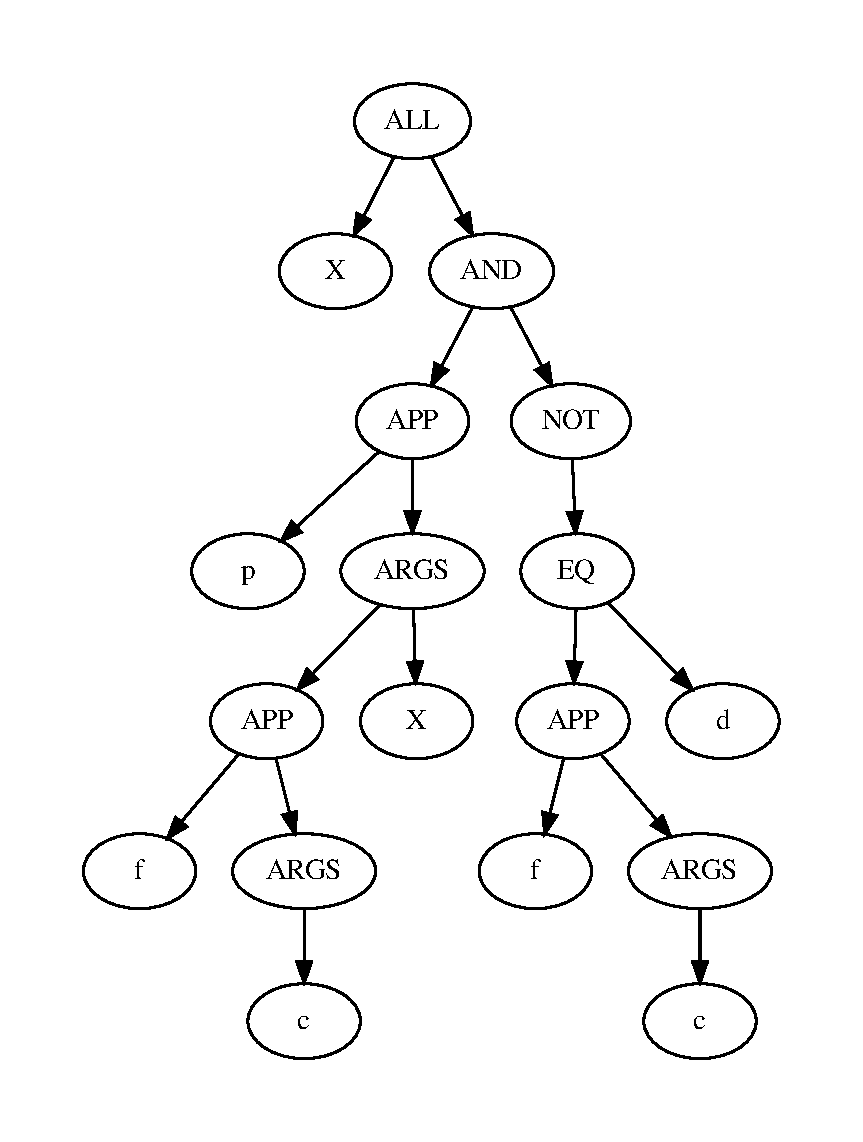
\includegraphics[width=\linewidth]{translation-ast}
		\caption{AST.}
	\end{subfigure}
%	\begin{subfigure}{.39\textwidth}
%%		\centering
%		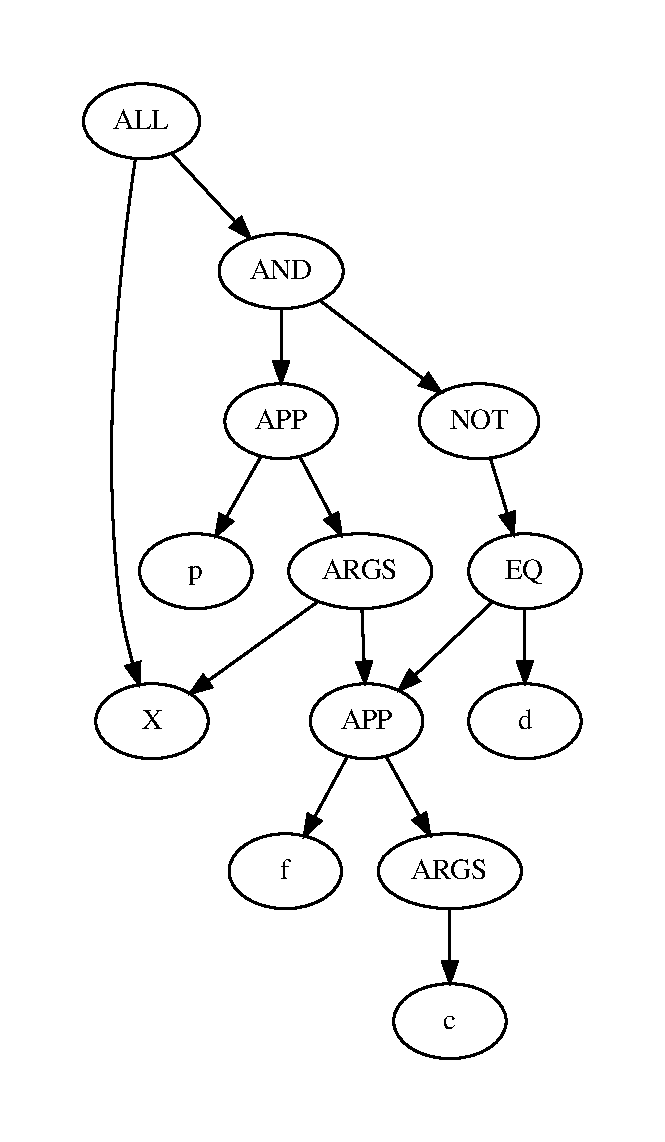
\includegraphics[width=\linewidth]{translation-graph}
%		\caption{De-duplicated DAG.}
%	\end{subfigure}
	\begin{subfigure}{.3\textwidth}
		\centering
		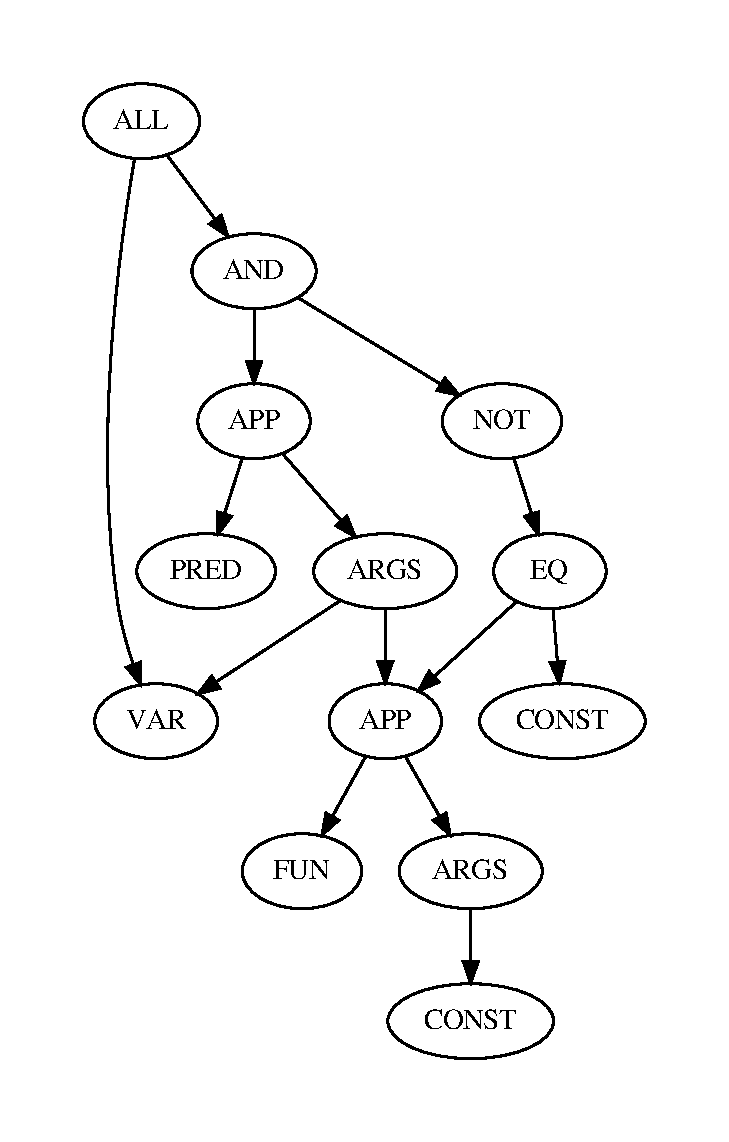
\includegraphics[width=\linewidth]{translation-nameless}
		\caption{Nameless DAG.}
	\end{subfigure}
	\begin{subfigure}{.25\textwidth}
		\centering
		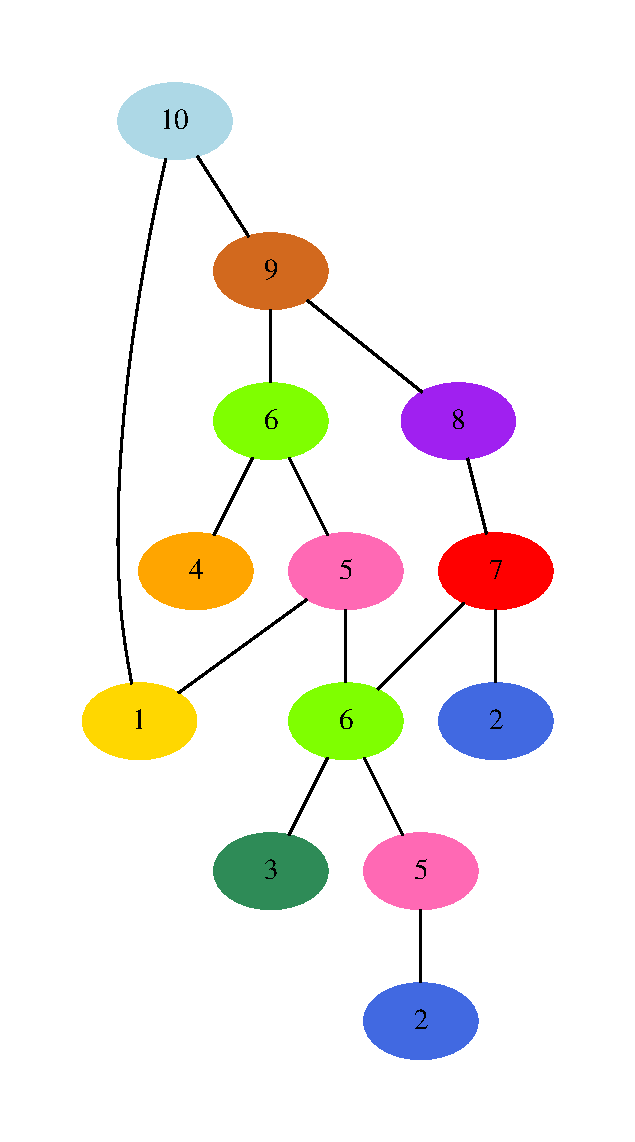
\includegraphics[width=\linewidth]{translation-undirected}
		\caption{Final result.}
	\end{subfigure}
	\caption{The translation process for \(\forall x. \left[p\left(f(c), x\right) \wedge \lnot\left(f(c) = d\right)\right]\) to a graph, as seen by the neural network.}
	\label{figure:translation}
\end{figure}

\subsection{Augmentation}
\label{section:augmentation}
One possible solution~\cite{imbalanced} to the problem of classification on imbalanced domains is to synthesise new data for under-represented classes --- in this case unsatisfiable formulae --- from existing data by augmenting it.
An example is augmenting image data by cropping, flipping or adding noise to existing images.
There are many possible ways to augment formulae graphs.
For this prototype, a simple approach is taken in which a small number of nonsense formulae are added to the graph by randomly adding nodes/edges where appropriate.
This approach has the advantage of exposing the network to ``noise'' such as additional axioms which might well occur in practice, but if the network is adequately capable of filtering these then no new formulae are actually seen.

\subsection{Neural Architecture}
In a typical convolutional network architecture for images~\cite{cnn}, there are a series of filtering stages, followed by a densely-connected neural network.
Each filtering stage intuitively combines data from local features (via \emph{convolution}), then reduces the dimensions of the image (via \emph{pooling}) for the next stage.
Graph neural networks have analogous convolution~\cite{gcn} (combining information from neighbouring nodes) and pooling~\cite{top-k-pooling} (merging nodes to reduce the size of the input graph) operators.
A brief period of experimentation with these operators yielded the following network architecture, shown in Fig. \ref{figure:network}.
\begin{enumerate}
	\item Input. A graph \(G\) consisting of one-hot encoded nodes \(N\) and edges \(E\).
	\item Embedding. Each node is mapped to an embedding vector of size 64 via a trained dense embedding.
	\item Initial Convolution. 4 convolution layers are applied to the graph with rectified linear activations. This yields a graph of the same size, but with information exchanged between nodes.
	\item Convolution/Pooling. Similar convolution layers are then passed through \emph{top-\(k\)}~\cite{top-k-pooling} layers, retaining \(k = 60\%\) of the graph's nodes. This is repeated 3 times, reducing the size of the graph considerably.
	\item Convolution/Max-Pooling. A final convolution layer feeds into a max-pooling layer, combining all remaining node data into one datum, and dropping the edge data.
	\item Fully Connected. A fully-connected hidden layer with rectified linear activation halves the input size.
	\item Fully Connected/Softmax. A fully-connected final layer outputs two class labels, with softmax activation.
\end{enumerate}
It is not claimed that this is the optimal configuration, and no grid search has yet taken place to optimise the network architecture or hyper-parameters. 
To reduce over-fitting, dropout~\cite{dropout} is applied in convolutional and fully-connected layers, \(p = 0.1\).

\begin{figure}
	\centering
	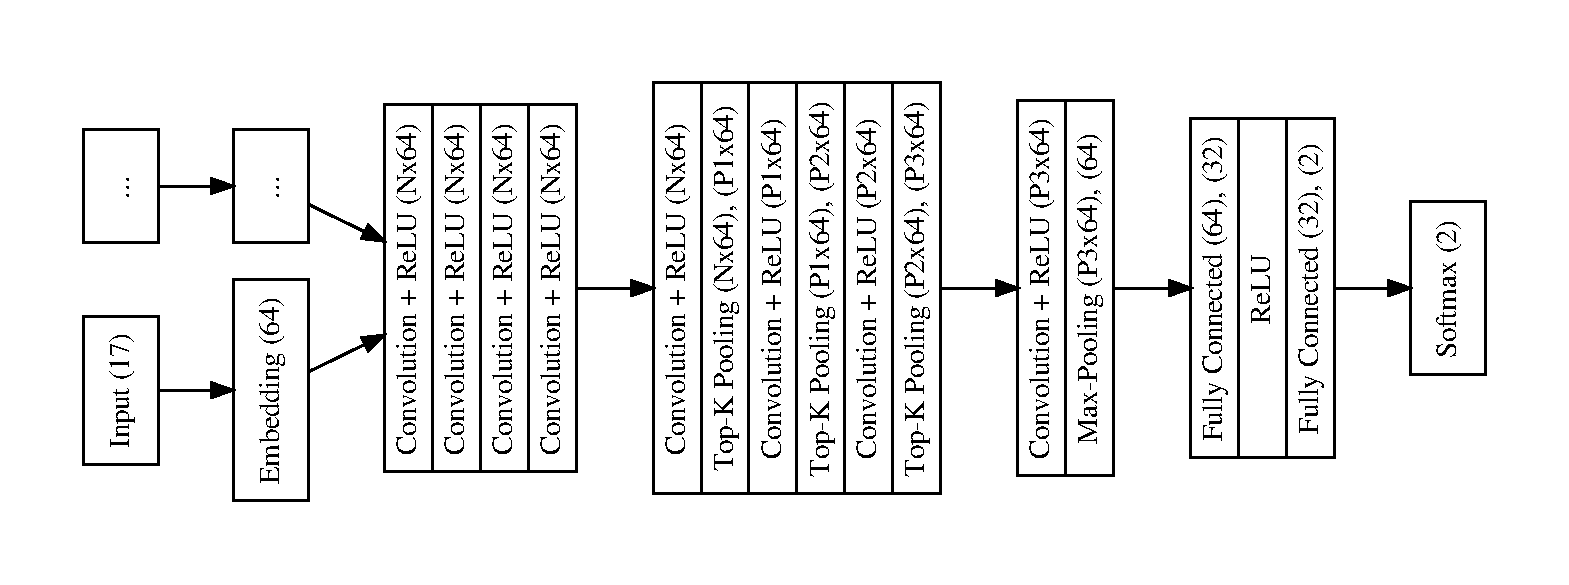
\includegraphics[width=\linewidth]{network}
	\caption{The neural network architecture. Initially there are \(N\) nodes, then after pooling there are \(P_1, P_2, P_3\) nodes. Node-level embedding layers are shown per-node, graph-level convolutional and pooling layers are shown per-graph.}
	\label{figure:network}
\end{figure}

\subsection{Implementation and Training}
This architecture was implemented with the PyTorch~\cite{pytorch} neural network library, combined with a graph-processing (``geometric'') extension library, PyTorch Geometric~\cite{pytorch-geometric}, which together provide facilities for automatic differentiation, GPU-accelerated training, pre-programmed layers for graph processing, and various utilities.
The dataset is split into a large training set and a smaller test set (200 balanced examples), since unsatisfiable examples were time-consuming to obtain in this setting.
The unsatisfiable training data were then augmented as described in section \ref{section:augmentation} to produce a balanced total training set of 3.5 million examples.
The network was trained on commodity desktop hardware with a mid-range GPU~\footnote{NVIDIA\textsuperscript{\textregistered} GeForce\textsuperscript{\textregistered} GT 730.} for 8 epochs/24 hours, optimising a negative log-likelihood loss function.

\begin{figure}
	\centering
	\captionsetup[subfigure]{justification=centering}
	\begin{subfigure}{.3\textwidth}
		\centering
		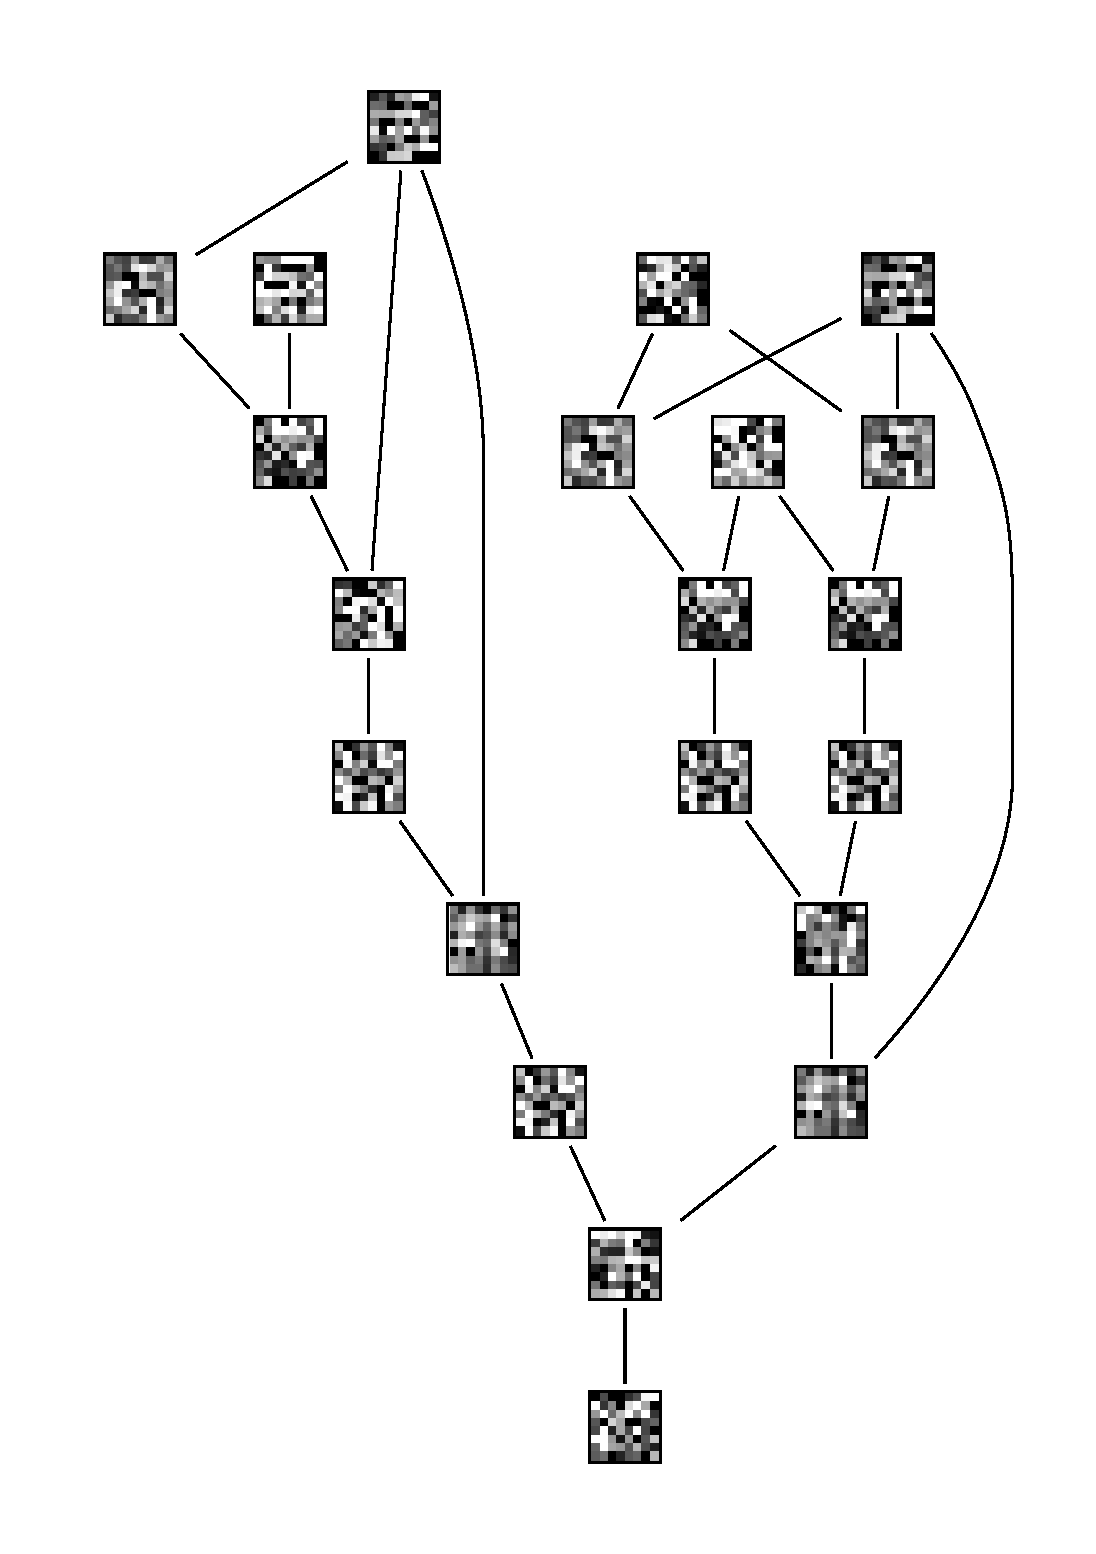
\includegraphics[width=\linewidth]{embedding}
		\caption{Output of embedding layer.}
	\end{subfigure}
	\begin{subfigure}{.3\textwidth}
		\centering
		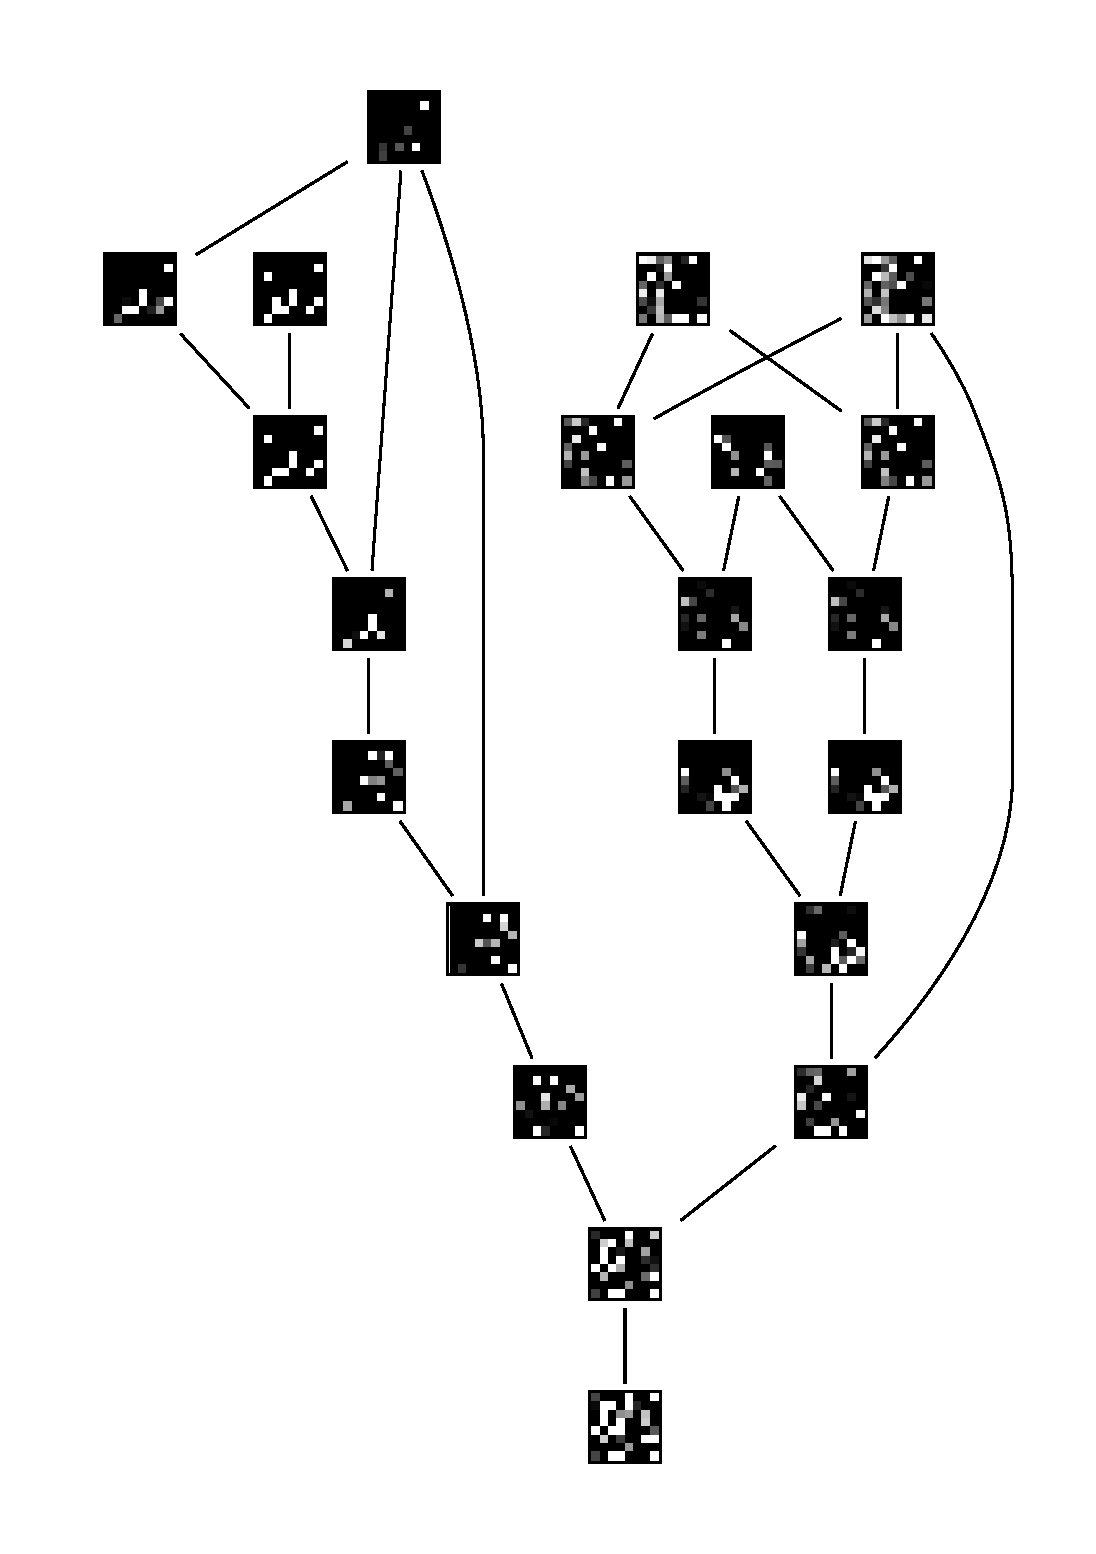
\includegraphics[width=\linewidth]{conv}
		\caption{Output after initial convolutions.}
	\end{subfigure}
	\begin{subfigure}{.3\textwidth}
		\centering
		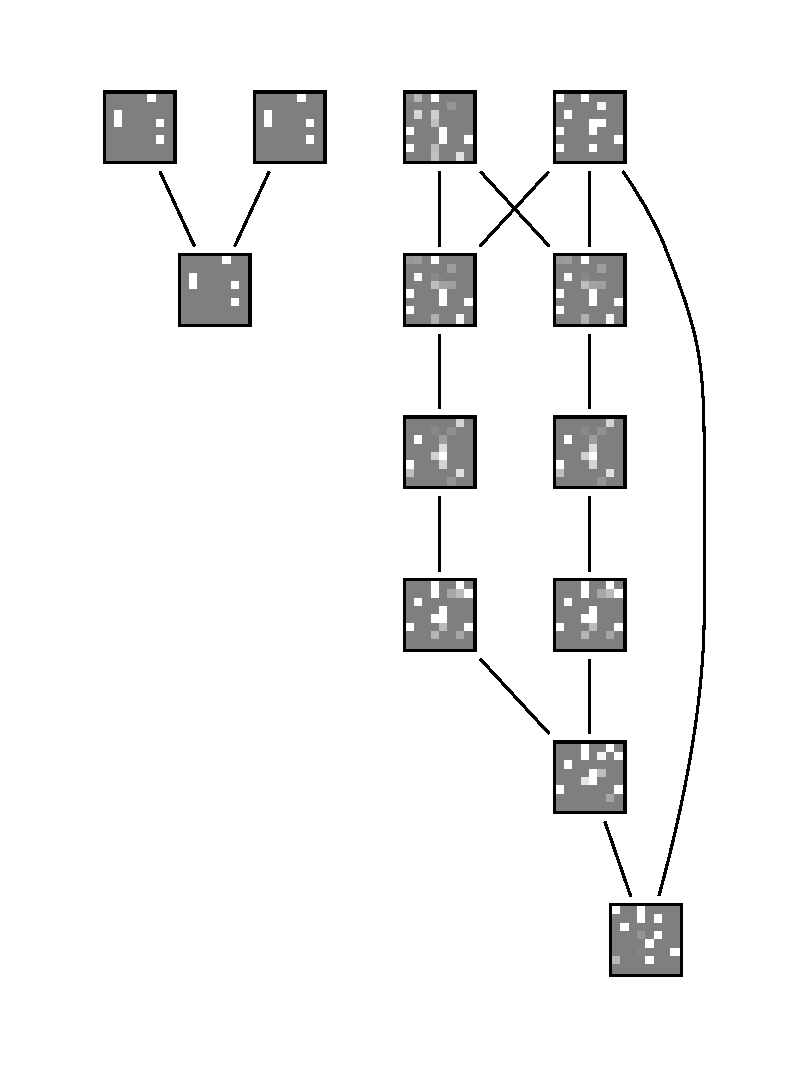
\includegraphics[width=\linewidth]{pool0}
		\caption{After first pooling.}
	\end{subfigure}
	\begin{subfigure}{.5\textwidth}
		\centering
		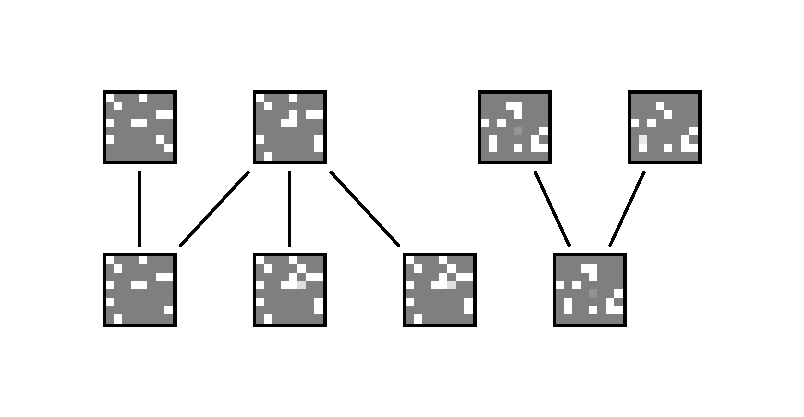
\includegraphics[width=\linewidth]{pool1}
		\caption{After second pooling.}
	\end{subfigure}
	\begin{subfigure}{.3\textwidth}
		\centering
		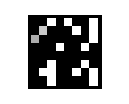
\includegraphics[width=\linewidth]{fc0}
		\caption{After max-pooling.}
	\end{subfigure}
	\caption{Computation in the neural network, showing intermediate values involved in the network (correctly) predicting the satisfiability of an input formula.}
	\label{figure:computation}
\end{figure}

\subsection{Network Evaluation}
The network was evaluated on the balanced test set of 200 examples, as described.
Various metrics for accuracy are shown in Table \ref{table:network-evaluation}.
While these results are very promising, it should be emphasised that it is unclear how effective a train/test split is in this setting (since similar subgoals may occur in both sets, even with proper data hygiene), and that this network is not attempting to determine the satisfiability of arbitrary formulae, merely those that occur in proof attempts on the \mizarlarge{} dataset.
The higher precision and lower recall values are likely an artefact of the augmentation process.
However, even with these caveats, the network performance is surprising and is practically useful for improving proof search in this dataset.

\begin{table}[t]
	\caption{Accuracy metrics for the neural heuristic.}
	\centering
	\begin{tabular}{r | c}
		\textbf{Metric} & \textbf{Score}\\
		\hline
		Accuracy & 93.0\%\\
		Precision&0.990\\	
		Recall&0.884\\
		\(F_1\)&0.934\\			
	\end{tabular}
	\quad
	\begin{tabular}{r | c}
		\textbf{Metric} & \textbf{Score}\\
		\hline
		True Positive&99\\
		True Negative&87\\
		False Positive&13\\		
		False Negative&1\\
	\end{tabular}	
	\label{table:network-evaluation}
\end{table}
%%%%%%%%%%%%%%%%%%%%%%%%%%%%%%%%%%%%%%%%%%%%%%%%%%%%%%%%%%%%%%
\section{Experimental Results}
\label{section:results}

To show that neural guidance can improve the performance of \lerna{} the system was run with and without guidance for 10 seconds on all available CPU cores.
All results were collected on commodity desktop hardware\footnote{Intel\textsuperscript{\textregistered} Core\textsuperscript{\texttrademark} i7-6700 CPU @ 3.40GHz, 16GB RAM.}.

%\subsection{Benchmark Results}
Table \ref{table:m2k-results} shows the total number of theorems proved using various configurations of \z3 and \lerna{} on the \mizarsmall{} dataset.
\z3 ran for a full 10 seconds to establish baseline performance, then as an oracle for 20 milliseconds to determine the number of ``trivial'' problems.
\lerna{} ran on an identical dataset, first without guidance from the neural heuristic, then with guidance.
%
\begin{table}[t]
	\caption{Total successful proof attempts on the \mizarsmall{} dataset.}
	\centering
	\begin{tabular}{r | c}
		\textbf{Configuration} & \textbf{Proofs}\\
		\hline
		\z3 (10s, as baseline) & 1216\\
		\z3 (20ms, as oracle) & 711\\
		\lerna{}, unguided (10s, with oracle) & 969\\
		\lerna{}, guided (10s, with oracle) & 1023\\
	\end{tabular}
	\label{table:m2k-results}
\end{table}
%
With neural guidance \lerna{} was able to solve an additional 54 problems and overall \lerna{} was shown to be complementary to \z3{}, proving 114 problems that \z3{} was unable to solve on its own. Conversely, \z3{} was able to solve more problems in total, which unsurprising given the maturity of the tool. These results show that \lerna{} is able to learn from experience and complement an existing ATP.

%Although clearly worse, \lerna{} solves a significantly different set of problems compared to the baseline: 114 problems are uniquely solved by \lerna{}.
%It should be noted that the impressive results reported by the rlCoP system~\cite{rlCoP} are not directly comparable here due to differences in experimental setup.


%%%%%%%%%%%%%%%%%%%%%%%%%%%%%%%%%%%%%%%%%%%%%%%%%%%%%%%%%%%%%%
\section{Future Work}

Given the prototype nature of this work, we have included a detailed discussion on future directions. 
%The style of theorem prover described opens many new directions for future work and improvements to the system.
As \lerna{} is a very new system, there is likely much to be gained by simple engineering and tuning: for example, the UCT exploration parameter \(c\) has been left at its theoretical optimum value \(\sqrt{2}\), but it is likely that a higher value will account for neural network inaccuracies and hence improve performance.
Training on, benchmarking with, and optimising for other datasets (such TPTP or SMT-LIB) is also left as future work.

\paragraph{Proof Search}
\lerna{} is well-suited for long-term proof search attempts in mathematics, such as those employed in the AIM project~\cite{AIM}: search is stable over time and does not produce a combinatorial explosion in the same way that some traditional systems tend to after a short period.
Additionally, the amount of information (``confidence'') in the system grows over time, as a result of a growing number of oracle invocations and neural network evaluations.
Proof search can in principle be manually inspected more easily than in saturation-based provers to examine promising subgoals and remove known falsehoods from the search space.
The authors hope to explore applying the system to this interesting domain. 

Another future direction for proof search is a principled incomplete mode where branches deemed sufficiently uninteresting by the heuristic are pruned, perhaps in response to resource constraints as in limited resource strategies~\cite{LRS}.
This approach, while clearly incomplete, would significantly accelerate proof search in the direction of more promising search within the available resources.

\paragraph{Prover Calculus}
The calculus currently employed is deliberately na\"ive and extensions should be explored. 
In particular, the simplification routines can be improved to remove more trivial sub-formulae as, while in general the oracles' preprocessing will remove these, they serve as noise for the neural network and might also increase the number of inference steps required to reach a proof.
As one possible view of this approach is as an intelligent preprocessor for an existing ATP, more aggressive and/or weakening inferences might be included in the calculus.
For instance, \emph{prenexing} (or conversely \emph{miniscoping}) formulae can have a significant effect on proof search for some theorem provers, so including suitable quantifier-manipulation rules might prove to be a useful extension.

Ideas from other refutation-tableaux calculi could well be suitable for this system.
The authors are attempting to integrate an adapted connection rule from the non-clausal connection calculus~\cite{non-clausal-connections}, as used in nanoCoP~\cite{nanocop}, in order to reduce the number of proof steps required to instantiate universal quantifiers.
Finally, this prover architecture can support other logics without excessive modification.
Given that \z3 is already capable of supporting many \emph{theories}, such as arithmetic or datatypes, a many-sorted first order logic such as those described by SMTLIB or the TFF0 dialect of TPTP seems appropriate.

\paragraph{Oracle}
While \z3 is a strong theorem prover in its own right and performs well here, it remains to be seen if it is the best for this application.
Other ATPs (or counter-example-finding systems) should be explored. 
A \emph{portfolio} of several oracle systems working in tandem might also be considered, although of course this will eventually retard proof search linearly in the number of systems present.
Reducing the number of oracle invocations is another area for optimisation.
Currently, the system calls an oracle for every new sub-goal generated.
It seems unlikely that the sub-goal is materially easier to dispatch than its parent (especially in the case of propositional inferences that do not split the goal), so heuristically or probabilistically removing such subgoals from the oracle's queue is a possible area for improvement.
\lerna{} does not currently use any information from the oracle beyond its status: using auxiliary information such as satisfying models or unused formulae could well aid proof search.

\paragraph{Machine-Learned Heuristic}
Many other graph-based neural architectures are possible.
PyTorch Geometric alone currently includes nearly 40 other graph-specific neural layers pre-programmed from the literature\footnote{\url{https://rusty1s.github.io/pytorch_geometric/build/html/modules/nn.html}}.
Neural models specifically for theorem proving are relatively under-studied.
To combat this, data used for this paper will be published in the near future so that the machine-learning community can improve upon our simple models.
Different approaches to formula-to-graph translation, symbol embeddings, data augmentation, and model integration may also be explored.

%%%%%%%%%%%%%%%%%%%%%%%%%%%%%%%%%%%%%%%%%%%%%%%%%%%%%%%%%%%%%%
\section{Conclusions}
The introduced prototype \lerna{} system successfully implements a theorem prover with a neural heuristic processing the entire proof state, structured as a graph.
After training on data automatically generated by the prover system, the neural network approach is shown to be practically useful for improving proof search performance.
A number of approaches (batching, oracle invocations, parallelism) are employed to improve system efficiency.
While the prototype is not yet a successful state-of-the-art ATP, it has some unique desirable properties, among them simplicity, parallelism, parametricity with respect to calculus/oracle/heuristic, and introspection of proof state.
The general approach is flexible and presently unexplored.

\paragraph{Acknowledgements}
The authors wish to thank Josef Urban and his group in \v{C}VUT, Prague for their help and encouragement with early iterations of this work, and for supplying the Mizar dataset used in this paper.
%\clearpage

\bibliographystyle{splncs04}
\bibliography{references}
\end{document}
